\documentclass[a4paper, 12pt]{report}
\usepackage{cmap}
\usepackage[T2A]{fontenc}
\usepackage[utf8]{inputenc}
\usepackage[english,russian]{babel}
\usepackage{listings}
\usepackage{amsmath}
\usepackage{float}
\usepackage{csquotes}
\usepackage{graphicx}
\graphicspath{ {./images/} }
\usepackage{xcolor}
\definecolor{buzzlightyear}{HTML}{8757A5}
\definecolor{grass}{HTML}{738D06}
\definecolor{literal}{HTML}{F18A2B}
\definecolor{commentcolor}{HTML}{8E908B}

\lstdefinestyle{habrstyle}{
	backgroundcolor=\color{white},
	commentstyle=\color{commentcolor},
	keywordstyle=\bfseries\color{buzzlightyear},
	numberstyle=\tiny\color{commentcolor},
	stringstyle=\color{grass},
	basicstyle=\ttfamily\footnotesize,
	breakatwhitespace=false,         
    	breaklines=true,                 
   	captionpos=b,                    
    	keepspaces=true,                 
    	numbers=left,                    
    	numbersep=7pt,                  
    	showspaces=false,                
    	showstringspaces=false,
   	showtabs=false,                  
    	tabsize=4
}

\lstset{style=habrstyle}

\author{3530901/80201, Шелаев Н. Р.}
\title{Лабораторная работа № 5. Автокорреляция.}
\date{\today}

\begin{document}
	\maketitle
	\tableofcontents
	\listoffigures
	\lstlistoflistings

	\chapter{Корреляция}
	Посмотрим на значение корреляции между двумя одинаковыми сигналами, сдвинутыми по фазе.
	\begin{lstlisting}[language=Python,caption=Два сдвинутые по фазе сигнала]
		from thinkdsp import SinSignal

		def make_sine(offset):
			signal = SinSignal(freq = 440, offset = offset)
			wave = signal.make_wave(duration=0.5, framerate=10000)
			return wave
		
		def compute_corr(offset):
			wave1 = make_sine(offset = 0)
			wave2 = make_sine(offset = -offset)
			wave1.segment(duration = 0.01).plot()
			wave2.segment(duration = 0.01).plot()
			corr = wave1.corr(wave2)
			print('corr =', corr)
			decorate(xlabel='Time (s)')
		
		PI2 = np.pi * 2
		slider = widgets.FloatSlider(min = 0, max = PI2, value = 1)
		interact(compute_corr, offset = slider);
	\end{lstlisting}
	\begin{figure}[H]
		\centering
		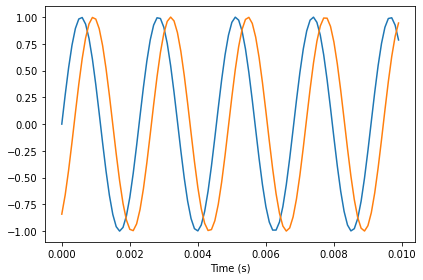
\includegraphics[width=0.75\textwidth]{sin1.png}
		\caption{Изменение фазы между двумя одинаковыми сигналами}
		\label{fig:sin1}
	\end{figure}
	\begin{lstlisting}[language=Python,caption=Корреляция между сигналами в зависимости от фазы]
		offsets = np.linspace(0, PI2, 101)
		corrs = []
		for offset in offsets:
			wave2 = make_sine(offset)
			corr = np.corrcoef(wave1.ys, wave2.ys)[0, 1]
			corrs.append(corr)
	
		plt.plot(offsets, corrs)
	\end{lstlisting}
	\begin{figure}[H]
		\centering
		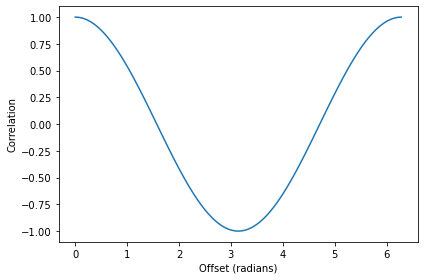
\includegraphics[width=0.75\textwidth]{sin2.png}
		\caption{И получили ... косинусоиду}
		\label{fig:sin2}
	\end{figure}
	Корреляция между сигналами в одной фазе равна 1, в противофазе она становится равна -1.

	\chapter{Последовательная корреляция}
	Построим последовательную корреляцию для различных видов шума.
	\begin{lstlisting}[language=Python,caption=Некоррелированный шум]
		from thinkdsp import UncorrelatedGaussianNoise		

		def serial_corr(wave, lag = 1):
    			N = len(wave)
    			y1 = wave.ys[lag:]
    			y2 = wave.ys[:N-lag]
    			corr = np.corrcoef(y1, y2)[0, 1]
			return corr
				
		signal = UncorrelatedGaussianNoise()
		wave = signal.make_wave(duration=0.5, framerate=11025)
		serial_corr(wave)
	\end{lstlisting}
	Значение корреляции близко к 0 (кто бы мог подумать?).
	\begin{lstlisting}[language=Python,caption=Броуновский шум]
		from thinkdsp import BrownianNoise

		signal = BrownianNoise()
		wave = signal.make_wave(duration=0.5, framerate=11025)
		serial_corr(wave)
	\end{lstlisting}
	Значение корреляции близко к 1 (тоже ничего удивительного).
	\begin{lstlisting}[language=Python,caption=Розовый шум]
		from thinkdsp import PinkNoise

		signal = PinkNoise(beta = 1)
		wave = signal.make_wave(duration=0.5, framerate=11025)
		serial_corr(wave)
	\end{lstlisting}
	В этот раз значение корреляции близко к 0,8.
	\begin{lstlisting}[language=Python,caption=Немного более подробно изучим Розовый шум]
		np.random.seed(25)
		betas = np.linspace(0, 2, 21)
		corrs = []

		for beta in betas:
			signal =  PinkNoise(beta = beta)
			wave = signal.make_wave(duration=1.0, framerate=11025)
			corr = serial_corr(wave)
			corrs.append(corr)
    
		plt.plot(betas, corrs)
	\end{lstlisting}
	\begin{figure}[H]
		\centering
		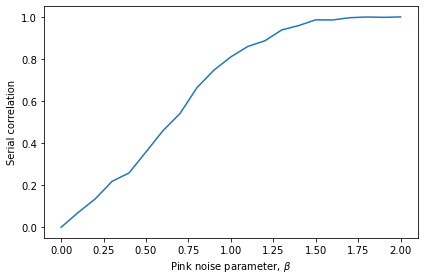
\includegraphics[width=0.75\textwidth]{beta1.png}
		\caption{Зависимость значения корреляции от значения параметра}
		\label{fig:beta1}
	\end{figure}
	\begin{lstlisting}[language=Python,caption=Функция автокорреляции для Розового шума]
		def autocorr(wave):
			lags = np.arange(len(wave.ys) // 2)
			corrs = [serial_corr(wave, lag) for lag in lags]
			return lags, corrs
		
		def plot_pink_autocorr(beta, label):
			signal = PinkNoise(beta = beta)
			wave = signal.make_wave(duration=1.0, framerate=10000)
			lags, corrs = autocorr(wave)
			plt.plot(lags, corrs, label = label)

		np.random.seed(25)

		for beta in [1.7, 1.0, 0.3]:
			label = r'$\beta$ = %.1f' % beta
			plot_pink_autocorr(beta, label)
	\end{lstlisting}
	\begin{figure}[H]
		\centering
		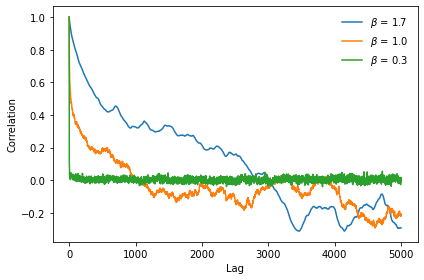
\includegraphics[width=0.75\textwidth]{beta2.png}
		\caption{Зависимость корреляции от начальной фазы сигнала}
		\label{fig:beta2}
	\end{figure}
	При низких значениях $\beta$ корреляция быстро падает. По мере увеличения $\beta$ эта зависимость длится дольше.

	\chapter{Автокорреляция периодических сигналов}
	Теперь изучим автокорреляцию разных периодических сигналов.
	\begin{lstlisting}[language=Python,caption=Запись вокального исполнения чирпов]
		from thinkdsp import read_wave

		wave = read_wave('28042__bcjordan__voicedownbew.wav')
		wave.normalize()
		spectrum = wave.make_spectrum()
		spectrum.plot()
		spectro = wave.make_spectrogram(seg_length = 1024)
		spectro.plot(high = 4200)
	\end{lstlisting}
	\begin{figure}[H]
		\centering
		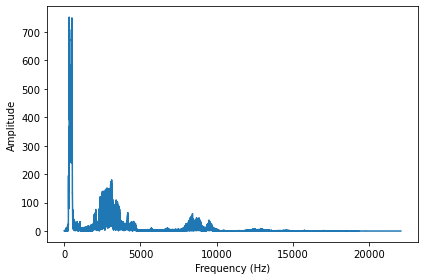
\includegraphics[width=0.75\textwidth]{acr1.png}
		\caption{Спектр данного сигнала}
		\label{fig:arc1}
	\end{figure}
	\begin{figure}[H]
		\centering
		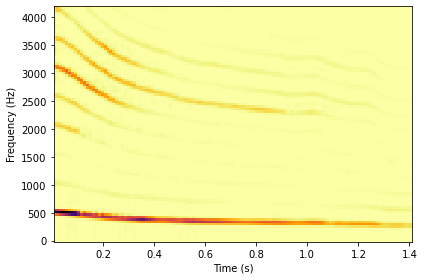
\includegraphics[width=0.75\textwidth]{acr2.png}
		\caption{Спектрограмма сигнала}
		\label{fig:arc2}
	\end{figure}
	\begin{lstlisting}[language=Python,caption=Уменьшение ширины сегмента]
		duration = 0.01
		segment = wave.segment(start=0.2, duration=duration)
		segment.plot()
		spectrum = segment.make_spectrum()
		spectrum.plot(high = 1000)
	\end{lstlisting}
	\begin{figure}[H]
		\centering
		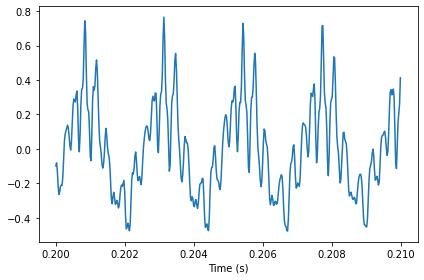
\includegraphics[width=0.75\textwidth]{acr3.png}
		\caption{Полученный сегмент сигнала}
		\label{fig:arc3}
	\end{figure}
	\begin{figure}[H]
		\centering
		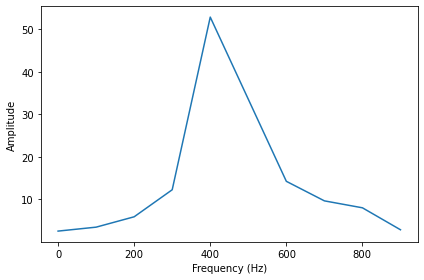
\includegraphics[width=0.75\textwidth]{acr4.png}
		\caption{Спектр этого сегмента}
		\label{fig:arc4}
	\end{figure}
	\begin{lstlisting}[language=Python,caption=Функция для нахождения корреляции между сигналами]
		def plot_shifted(wave, offset = 0.001, start = 0.2):
			segment1 = wave.segment(start=start, duration=0.01)
			segment1.plot(linewidth = 2, alpha = 0.8)
			segment2 = wave.segment(start=(start - offset), duration=0.01)
			segment2.shift(offset)
			segment2.plot(linewidth = 2, alpha = 0.4)
			corr = segment1.corr(segment2)
			text = r'$\rho =$ %.2g' % corr
			plt.text((segment1.start + 0.0005), -0.8, text)
			decorate(xlabel = 'Time (s)')

		slider1 = widgets.FloatSlider(min = 0, max = 0.004, step = (0.004 / 40), value = 0)
		slider2 = widgets.FloatSlider(min = 0.1, max = 0.5, step = 0.05, value = 0.2)
		interact(plot_shifted, wave = fixed(wave), offset = slider1, start = slider2);
	\end{lstlisting}
	\begin{figure}[H]
		\centering
		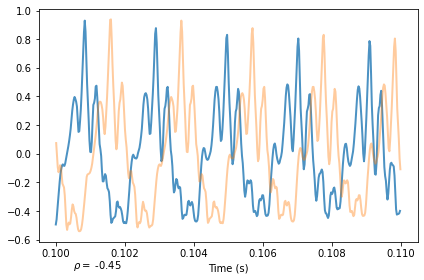
\includegraphics[width=0.75\textwidth]{acr5.png}
		\caption{Зависимость значения корреляции от фазы}
		\label{fig:arc5}
	\end{figure}
	\begin{lstlisting}[language=Python,caption=Автокорреляция чирпа]
		wave = read_wave('28042__bcjordan__voicedownbew.wav')
		wave.normalize()
		duration = 0.01
		segment = wave.segment(start=0.2, duration=duration)
		lags, corrs = autocorr(segment)
		plt.plot(lags, corrs)
	\end{lstlisting}
	\begin{figure}[H]
		\centering
		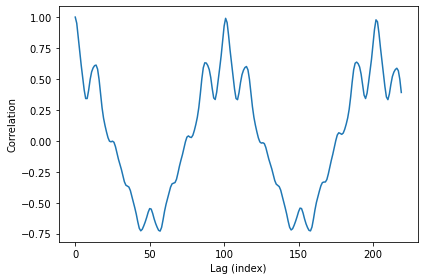
\includegraphics[width=0.75\textwidth]{acr6.png}
		\caption{Зависимость корреляции от начальной фазы сигнала}
		\label{fig:arc6}
	\end{figure}

	\chapter{Встроенная функция автокорреляции}
	Поспользуемся встроенной функцией автокорреляции в модуле \texttt{NumPy}.
	\begin{lstlisting}[language=Python,caption=Использование встроенной функции для автокорреляции]
		N = len(segment)
		corrs2 = np.correlate(segment.ys, segment.ys, mode = 'same')
		lags = np.arange(-N // 2, N // 2)
		plt.plot(lags, corrs2)
	\end{lstlisting}
	\begin{figure}[H]
		\centering
		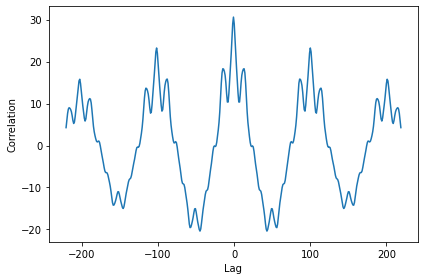
\includegraphics[width=0.75\textwidth]{acr7.png}
		\caption{Полученная зависимость}
		\label{fig:arc7}
	\end{figure}
	\begin{lstlisting}[language=Python,caption=Правая часть сигнала]
		N = len(corrs2)
		lengths = range(N, N // 2, -1)
		half = corrs2[N // 2:].copy()
		half /= lengths
		half /= half[0]
		plt.plot(half)
	\end{lstlisting}
	\begin{figure}[H]
		\centering
		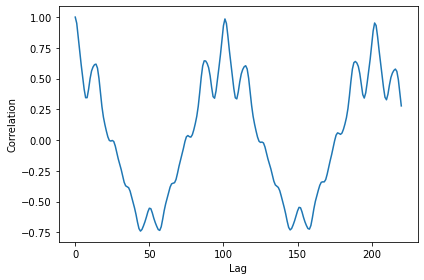
\includegraphics[width=0.75\textwidth]{acr8.png}
		\caption{Взяли правую часть сигнала (фаза > 0)}
		\label{fig:arc8}
	\end{figure}
	\begin{lstlisting}[language=Python,caption=Сравнение двух функций]
		plt.plot(half)
		plt.plot(corrs)	
		diff = corrs - half[:-1]
		plt.plot(diff)
	\end{lstlisting}
	\begin{figure}[H]
		\centering
		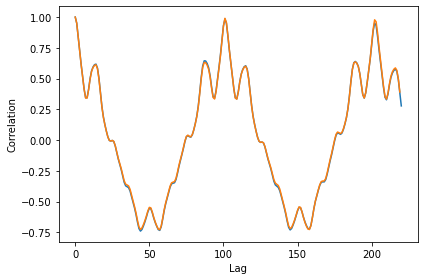
\includegraphics[width=0.75\textwidth]{acr9.png}
		\caption{Сравнение полученных результатов двух различных функций автокорреляции}
		\label{fig:arc9}
	\end{figure}
	\begin{figure}[H]
		\centering
		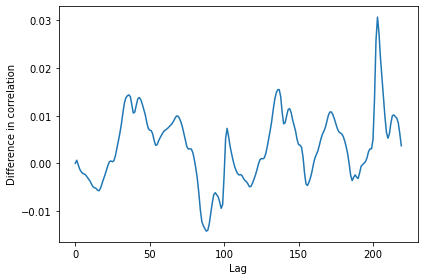
\includegraphics[width=0.75\textwidth]{acr10.png}
		\caption{Разница между результатами двух функций}
		\label{fig:arc10}
	\end{figure}
	Результаты работы этих двух функций очень похожи, но встроенная функция работает быстрее.
	
	\chapter{Упражнения}
	\section{Задание 2}
	Создание итоговой функции для оценки основной частоты периодического сигнала.
	\begin{lstlisting}[language=Python,caption=Итоговая функция]
		from thinkdsp import read_wave

		wave = read_wave('28042__bcjordan__voicedownbew.wav')
		wave.normalize()
		wave.make_spectrogram(2048).plot(high = 4200)

		def estimate_fundamental(segment, low=70, high=150):
			lags, corrs = autocorr(segment)
			lag = np.array(corrs[low:high]).argmax() + low
			period = lag / segment.framerate
			frequency = 1 / period
			return frequency
	\end{lstlisting}
	\begin{figure}[H]
		\centering
		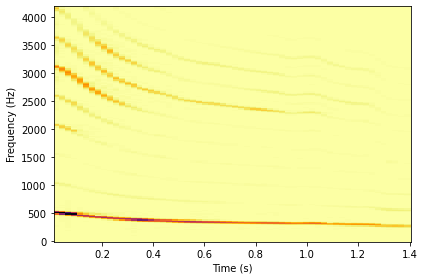
\includegraphics[width=0.75\textwidth]{test1.png}
		\caption{Спектрограмма сигнала}
		\label{fig:test1}
	\end{figure}
	\begin{lstlisting}[language=Python,caption=Проверка работы функции]
		step = 0.05
		starts = np.arange(0.0, 1.4, step)
		ts = []
		freqs = []
		for start in starts:
			ts.append(start + step / 2)
			segment = wave.segment(start=start, duration=duration)
			freq = estimate_fundamental(segment)
			freqs.append(freq)
		wave.make_spectrogram(2048).plot(high = 900)
		plt.plot(ts, freqs, color = 'white')
	\end{lstlisting}
	\begin{figure}[H]
		\centering
		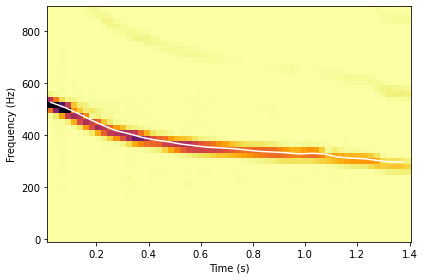
\includegraphics[width=0.75\textwidth]{test2.png}
		\caption{Полученная спектрограмма}
		\label{fig:test2}
	\end{figure}
	
	\section{Задание 3}
	Автокорреляция цен в платежной системе \texttt{BitCoins}.
	\begin{lstlisting}[language=Python,caption=Метод Бартлетта]
		import pandas as pd
		from thinkdsp import Wave

		df = pd.read_csv('BTC_USD_2013-10-01_2020-03-26-CoinDesk.csv', parse_dates = [0])
		ys = df['Closing Price (USD)']
		ts = df.index
		wave = Wave(ys, ts, framerate = 1)
		wave.plot()
		lags, corrs = autocorr(wave)
		plt.plot(lags, corrs)
	\end{lstlisting}
	\begin{figure}[H]
		\centering
		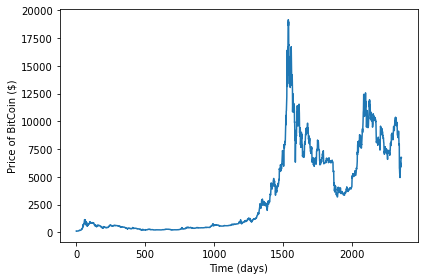
\includegraphics[width=0.75\textwidth]{bit1.png}
		\caption{Сигнал BitCoins}
		\label{fig:bit1}
	\end{figure}
	\begin{figure}[H]
		\centering
		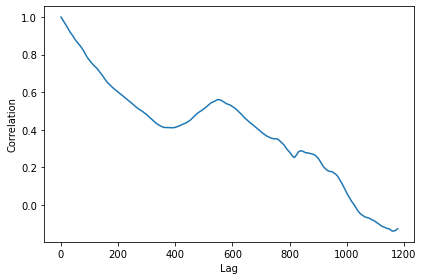
\includegraphics[width=0.75\textwidth]{bit2.png}
		\caption{Автокорреляция этого сигнала}
		\label{fig:bit2}
	\end{figure}
	\begin{lstlisting}[language=Python,caption=Снова сравним две функции]
		N = len(wave)
		corrs2 = np.correlate(wave.ys, wave.ys, mode='same')
		lags = np.arange(-N // 2, N // 2)
		N = len(corrs2)
		half = corrs2[N // 2:]
		lengths = range(N, N // 2, -1)
		half /= lengths
		half /= half[0]
		plt.plot(corrs, label = 'autocorr')
		plt.plot(half, label = 'correlate')
	\end{lstlisting}
	\begin{figure}[H]
		\centering
		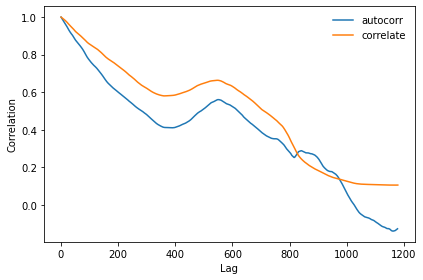
\includegraphics[width=0.75\textwidth]{bit3.png}
		\caption{Сравнение результатов работы двух функций}
		\label{fig:bit3}
	\end{figure}

	\section{Задание 4}
	Исследуем код в файле \texttt{saxophone.ipynb}.
	\begin{lstlisting}[language=Python,caption=Получение сигнала]
		wave=read_wave('100475__iluppai__saxophone-weep.wav')
		wave.normalize()
		gram = wave.make_spectrogram(seg_length = 1024)
		gram.plot(high = 3000)
	\end{lstlisting}
	\begin{figure}[H]
		\centering
		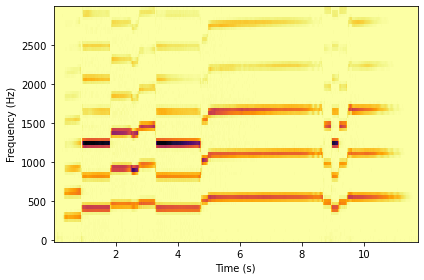
\includegraphics[width=0.75\textwidth]{sax1.png}
		\caption{Спектрограмма сигнала}
		\label{fig:sax1}
	\end{figure}
	\begin{lstlisting}[language=Python,caption=Продолжаем исследование]
		start = 2.0
		duration = 0.5
		segment = wave.segment(start = start, duration = duration)
		spectrum = segment.make_spectrum()
		spectrum.plot(high = 3000)
	\end{lstlisting}
	\begin{figure}[H]
		\centering
		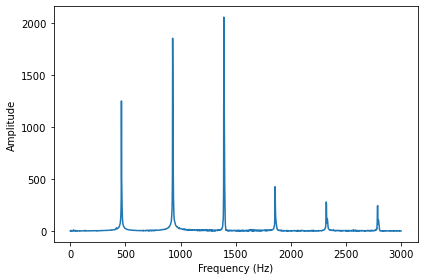
\includegraphics[width=0.75\textwidth]{sax2.png}
		\caption{Спектр сигнала}
		\label{fig:sax2}
	\end{figure}
	Пики спектра находятся на частотах 1392, 928 и 464 Гц.
	\begin{lstlisting}[language=Python,caption=Новая функция для автокорреляции]
		def autocorr_new(segment):
			corrs = np.correlate(segment.ys, segment.ys, mode = 'same')
			N = len(corrs)
			lengths = range(N, N // 2, -1)
			half = corrs[N // 2:].copy()
			half /= lengths
			half /= half[0]
			return half
		
		corrs = autocorr_new(segment)
		plt.plot(corrs[:200])
	\end{lstlisting}
	\begin{figure}[H]
		\centering
		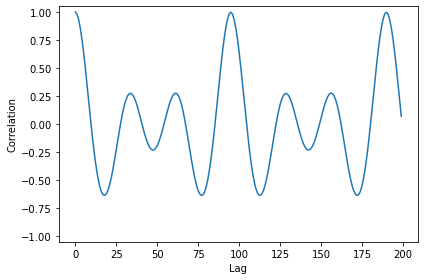
\includegraphics[width=0.75\textwidth]{sax3.png}
		\caption{График корреляции}
		\label{fig:sax3}
	\end{figure}
	\begin{lstlisting}[language=Python,caption=Применили ФВЧ]
		def find_frequency(corrs, low, high):
			lag = np.array(corrs[low:high]).argmax() + low
			period = lag / segment.framerate
			frequency = 1 / period
			return frequency
		
		find_frequency(corrs, 80, 100)
		spectrum2 = segment.make_spectrum()
		spectrum2.high_pass(600)
		spectrum2.plot(high = 3000)
		corrs = autocorr_new(segment2)
		plt.plot(corrs[:200])
	\end{lstlisting}
	\begin{figure}[H]
		\centering
		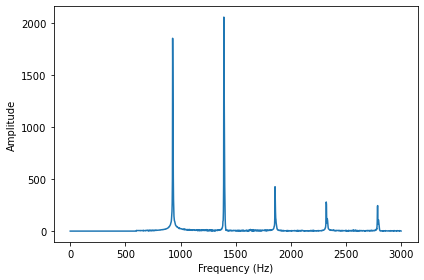
\includegraphics[width=0.75\textwidth]{sax4.png}
		\caption{Спектр сигнала после применения ФВЧ}
		\label{fig:sax4}
	\end{figure}
	\begin{figure}[H]
		\centering
		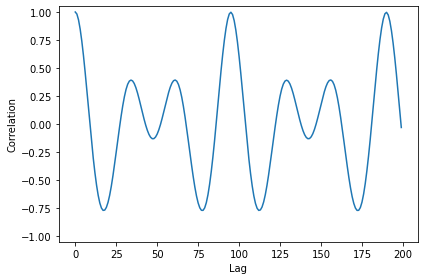
\includegraphics[width=0.75\textwidth]{sax5.png}
		\caption{Снова применили функцию автокорреляции}
		\label{fig:sax5}
	\end{figure}
	\begin{lstlisting}[language=Python,caption=Применили ФВЧ и ФНЧ]
		spectrum4 = segment.make_spectrum()
		spectrum4.high_pass(600)
		spectrum4.low_pass(1200)
		spectrum4.plot(high = 3000)
		corrs = autocorr_new(segment4)
		plt.plot(corrs[:200])
	\end{lstlisting}
	\begin{figure}[H]
		\centering
		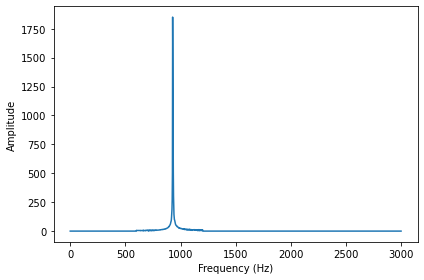
\includegraphics[width=0.75\textwidth]{sax6.png}
		\caption{Спектр сигнала после применения ФВЧ и ФНЧ}
		\label{fig:sax6}
	\end{figure}
	\begin{figure}[H]
		\centering
		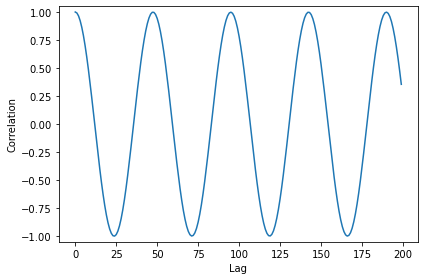
\includegraphics[width=0.75\textwidth]{sax7.png}
		\caption{Применили функцию автокорреляции}
		\label{fig:sax7}
	\end{figure}
	В результате, можно сделать вывод, что восприятие высоты тона не полностью основано на спектральном анализе, но также зависит и от автокорреляции.

	\chapter{Вывод}
	В данной работе мы изучили изменение корреляции от фазы одинаковых сигналов и посмотрели влияние функции автокорреляции на звучание различных сигналов.
\end{document}